% !TeX program = pdfLaTeX
\documentclass[12pt]{article}
\usepackage{amsmath}
\usepackage{graphicx,psfrag,epsf}
\usepackage{enumerate}
\usepackage{natbib}
\usepackage{textcomp}
\usepackage[hyphens]{url} % not crucial - just used below for the URL
\usepackage{hyperref}
\providecommand{\tightlist}{%
  \setlength{\itemsep}{0pt}\setlength{\parskip}{0pt}}

%\pdfminorversion=4
% NOTE: To produce blinded version, replace "0" with "1" below.
\newcommand{\blind}{0}

% DON'T change margins - should be 1 inch all around.
\addtolength{\oddsidemargin}{-.5in}%
\addtolength{\evensidemargin}{-.5in}%
\addtolength{\textwidth}{1in}%
\addtolength{\textheight}{1.3in}%
\addtolength{\topmargin}{-.8in}%

%% load any required packages here



% Pandoc citation processing

\usepackage{pdflscape}

\begin{document}


\def\spacingset#1{\renewcommand{\baselinestretch}%
{#1}\small\normalsize} \spacingset{1}


%%%%%%%%%%%%%%%%%%%%%%%%%%%%%%%%%%%%%%%%%%%%%%%%%%%%%%%%%%%%%%%%%%%%%%%%%%%%%%

\if0\blind
{
  \title{\bf An observational study of papers published in \emph{PLOS ONE} and
studies posted to a trial registry.}

  \author{
        Nicole White \thanks{The authors gratefully acknowledge computational resources and services
used in this work provided by the eResearch Office, Queensland
University of Technology, Brisbane, Australia.} \\
    School of Public Health and Social Work, QUT\\
     and \\     Thiru Balasubramaniam, Richi Nayak \\
    To add\\
     and \\     Adrian Barnett \\
    School of Public Health and Social Work, QUT\\
      }
  \maketitle
} \fi

\if1\blind
{
  \bigskip
  \bigskip
  \bigskip
  \begin{center}
    {\LARGE\bf An observational study of papers published in \emph{PLOS ONE} and
studies posted to a trial registry.}
  \end{center}
  \medskip
} \fi

\bigskip
\begin{abstract}
The text of your abstract. 200 or fewer words.
\end{abstract}

\noindent%
{\it Keywords:} 3 to 6 keywords, that do not appear in the title
\vfill

\newpage
\spacingset{1.45} % DON'T change the spacing!

\hypertarget{introduction}{%
\section{Introduction}\label{introduction}}

An ideal statistical analysis will use appropriate methods to create
insights from the data and inform the research questions. Unfortunately
many current statistical analyses are far from ideal, with many
researchers using the wrong methods, misinterpreting the results, or
failing to adequately check their assumptions \citep{2008, Leek2017}.
Some researchers take a ``mechanistic'' approach to statistics, copying
the few methods they know regardless of their appropriateness, and then
going through the motions of the analysis \citep{Stark2018}.

Many researchers lack adequate training in research methods, and
statistics is something they do with trepidation and even ignorance
\citep{Altman1994, King2019}. However, using the wrong statistical
methods can cause real harm \citep{Altman1994, Brown2018} and bad
statistical practices are being to used abet weak science
\citep{Stark2018}. Statistical mistakes are a key source of waste in
research and partly explain the current reproducibility crisis in
science \citep{Allison2016}. Even when the correct methods are used,
many researchers fail to describe them adequately, making it difficult
to reproduce the results \citep{Ernst2017, Zhou2018}. Poor statistical
methods might not be caught by reviewers, as they may not be qualified
to judge the statistics. A recent survey of editors found that only 23\%
of health and medical journals used expert statistical review for all
articles \citep{Hardwicke2020}, which was little different from a survey
from 22 years ago \citep{Goodman1998}.

There is guidance for researchers on how to write up their statistical
methods and results. The International Committee of Medical Journal
Editors recommend that researchers should: ``Describe statistical
methods with enough detail to enable a knowledgeable reader with access
to the original data to judge its appropriateness for the study and to
verify the reported results'' \citep{ICMJE2019}. More detailed guideance
is given by the SAMPL and EQUATOR guidelines
\citep{Lang2013, Altman2016} with the latter covering all apsects of the
paper. Both of these guidelines were led by Doug Altman, who spoke often
and for many years about the need for better statistical reporting. The
awareness and use of these guidelines could be improved. There were 256
Google Scholar citations to the SAMPL paper (as at 15 March 2021) which
is a good citation statistic for most papers, but is low considering the
millions of papers that use statistical analysis.

Two statisticians on this paper (AB and NW) have heard researchers admit
that they have copied-and-pasted their statistical methods sections from
other papers, regardless of whether they are appropriate. The aim of
this paper is to use text-mining methods to analyse the content of
statistical methods sections included in common research outputs.
Results are then evaluated to estimate the extent that researchers are
using cut-and-paste or `boilerplate' statistical methods sections.
Boilerplate text is that ``which can be reused in new contexts or
applications without significant changes to the original''
\citep{Wikipedia}. Use of these methods sections indicates that little
thought has gone into the statistical analysis.

\hypertarget{methods}{%
\section{Methods}\label{methods}}

\subsection{Data sources}

We used two openly available data sources to find statistical methods
sections: research articles published in \emph{PLOS ONE} and study
protocols registered on the Australian and New Zealand Clinical Trials
Registry (ANZCTR). Data sources were chosen as examples of common
research outputs that should include descriptions of statistical methods that
were used, or are planned, for analysing study outcomes.

\subsubsection{Public Library of Science (PLOS ONE)}
\label{sec:methodsPLOS}

\emph{PLOS ONE} is a large open access journal that publishes original
research across a wide range of scientific fields. Article submissions
are handled by an academic editor who selects peer reviewers based on
their self-nominated areas of expertise. Submissions do not undergo
formal statistical review. Instead, reviewers are required to assess
submissions against several publication criteria, including whether:
``Experiments, statistics, and other analyses are performed to a high
technical standard and are described in sufficient detail''
\citep{PLOS}. All reviewers are asked the question: ``Has the
statistical analysis been performed appropriately and rigorously?'',
with the possible responses of ``Yes'', ``No'' and ``I don't know''.

Authors are encouraged to follow published reporting guidelines such as
EQUATOR, to ensure that chosen statistical methods are appropriate for
the study design, and adequate details are provided to enable
independent replication of results.

All \emph{PLOS ONE} articles are freely accessible via the PLOS
Application Programming Interface (API). This enabled us to conduct
searches of full-text articles and analyse data on articles' text
content and general attributes such as publication date and field(s) of
research. To find papers with a statistical methods section we used
targeted API searches followed by article filtering based on section
headings. The data were downloaded on 3 July 2020.

\emph{Step 1: Targeted API searches}. API searches were completed using
the `rplos' package \citep{rplos}. Search queries targeted analysis-related terms, combining 
the words ``data'' or ``statistical'' with one of:
``analysis'', ``analyses'', ``method'', ``methodology'' or
``model(l)ing''. We allowed terms to appear anywhere in the article, to allow for the possibility of relevant text being placed in different
sections, for example, in the \emph{Material and Methods} section versus
\emph{Results}. Search results were indexed by a unique Digital Object
Identifier (DOI). Attribute data collected per DOI included journal
volume and subject classification(s).

\emph{Step 2: Partial matching on section headings}. Full text XML data
were downloaded and combined into a single dataset, organised by DOI and
subsection heading(s). Since \emph{PLOS ONE} does not prescribe
standardised headings to preface statistical methods sections, we
performed partial matching on available headings against frequently used
terms in initial search results: `Statistical analysis', `Statistical
analyses', `Statistical method', `Statistics', `Data analysis' and `Data
analyses'.

\subsubsection{Australia and New Zealand Clinical Trials Registry (ANZCTR)}
\label{sec:methodsANZCTR}

The ANZCTR was established in 2005 as part of a coordinated global
effort to improve research quality and transparency in clinical trials
reporting; observational studies can also be registered. All studies
registered on ANZCTR are publicly available and can be searched via an
online portal (\url{https://www.anzctr.org.au}).

Details required for registration follow a standardised template
\citep{ANZCTR}, which covers participant eligibility, the
intervention(s) being evaluated, study design and outcomes. The
information provided must be in English. Studies are not peer reviewed.

For the statistical methods section, researchers are asked to provide a
``brief description'' of the sample size calculations, statistical
methods and planned analyses, although this section is not compulsory
\citep{ANZCTR}. Studies are reviewed by ANZCTR staff for completeness of
key information, which does not include the completeness of the
statistical methods sections.

All studies available on ANZCTR were downloaded on 1 February 2020 in
XML format. We used all the text available in the ``Statistical
methods'' section. We also collated basic information about the study
including the study type (interventional or observational), submission
date, number of funders and target sample size. These variables were
chosen as we believed they might influence the completeness of the
statistical methods section, because we expected larger studies and
those with funding to be more complete, and we also were interested in
changes over time.

Studies prior to 2013 were excluded as the statistical methods section
appeared to be introduced in 2013. Some studies were first registered on
the alternative trial database \emph{clinicaltrials.gov} and then also
posted to ANZCTR. We excluded these studies because they almost all had
no completed statistical methods section as this section is not included
in \emph{clinicaltrials.gov}.

\subsection{Full-text processing}
\label{sec:methods-cleaning}

 Text cleaning aimed to standardise notation and
statistical terminology, whilst minimising changes to article style and
formatting. Datasets were cleaned using the `textclean package'
\citep{textclean}. \emph{R} code used for data extraction and cleaning is
available from \url{https://github.com/agbarnett/stats_section}.

Mathematical notation including Greek letters was converted from Unicode
characters to plain text. For example, the Unicode character
corresponding to \(\theta\) (\textless U+03B8\textgreater) was replaced
with `theta'. Common symbols outside of Unicode blocks including `\%'
(percent) and `\textless{}' (`less-than') were similarly converted into
plain text. General formatting was removed, this included carriage
returns, punctuation marks, in-text references (e.g.~``{[}42{]}'')
centred equations, and other non-ASCII characters. Text contained inside
brackets was retained to maximise content for analysis, with brackets
removed.

We compiled an extensive list of statistical terms to standardise
descriptions of statistical methods reported across both datasets. An
initial list was compiled by calculating individual word frequencies and
identifying relevant terms that appeared at least 100 times. Further
terms were sourced from index searches of three statistics textbooks
\citep{Diggle2013,Bland2015,Dobson2018}. The final list
is provided in Supplementary File 1. Plurals (e.g., `chi-squares')
unhyphenated (e.g., `chi square') and combined (e.g.~`chisquare') terms
were transformed to singular, hyphenated form (e.g., `chi-square').
Common statistical tests were also hyphenated (e.g., `hosmer lemeshow'
to `hosmer-lemeshow').

As a final step, common stop words including pronouns, contractions and
selected prepositions were removed. We retained selected stop words
that, if excluded, may have changed the context of statistical methods
being described, for example `between' and `against'.

\subsection{Clustering algorithm}

Let \(P \in R^{M \times N}\) denotes the paper content matrix where the
statistical methods sections of \(N\) papers consist of \(M\) distinct
terms. Text clustering for identifying common writing themes in these
papers requires this matrix to represent with a vector space model. Let
Matrix \(P\) be modeled with the unique terms in the processed sections
represented with the tf*idf (term frequent * inverse document frequency)
weighting schema to consider both common and rare terms.

Text clustering is known to face the curse of dimensionality due to the
high number of terms in doc\(\times\)term matrix representation
\citep{sutanto2018fine,aggarwal2012mining}. Therefore
text-based methods based on distance, density or probability face
difficulties
\citep{mohotti2018corpus,mohotti2019concept,park2018examining}.
Specifically, the distance difference between near and far points
becomes negligible in high-dimensional data \citep{aggarwal2012mining}.
This directly affects the distance-based methods such as
\textit{k}-means \citep{jain} in accurately identifying the common
subgroups. In addition, the sparseness of this high dimensional matrix
representation does not allow to differentiate the user groups based on
density differences
\citep{mohotti2018efficient,mohotti2018corpus}.

Non-negative Matrix factorization (NMF) which maps the high-dimensional
data to a lower-dimensional space has been found to provide an effective
solution by allowing to form clusters in the lower-dimensional space
\citep{luong2019clustering,kim2014algorithms}. NMF approximates
topic vectors in linear manner considering the context of terms.

In traditional NMF \citep{aggarwal2012mining}, the high-dimensional
matrix \(P \in R^{M \times N}\) is approximated by learning two factor
matrices \(W \in R^{M \times g}\) and \(H \in R ^{N \times g}\) where
\(g\) is the number of cluster groups or common topics in the data
collection, as follows.

\begin{equation}
\label{eq:2}
 P \approx WH^{T}
\end{equation}

The matrix factorization process approximates the lower dimensional
non-negative factor matrices \(W\) and \(H\) such that they can
represent high dimensional \(P\) with the least error. The objective
function in Eq \ref{eq:Eq2} iteratively attempts to update the entries
in \(W\) and \(H\) to find the optimum values which possess minimum sum
of square error for all the elements in both of those matrices. NMF uses
Frobenius norm as its objective function and will find the optimum value
of \textit{W} and \textit{H} iteratively.

\begin{equation}
\label{eq:Eq2}
\min \frac{1}{2}\|P - WH\|= \sum _{i=1}^{M}\sum _{j=1}^{N} \left(  P_{i,j} -\left(WH \right)_{i,j} \right)^{2}
\end{equation}

Matrix \textit{H} contains the information regarding topic membership of
each document. Topic membership of each method section in \(P\) is
obtained considering the maximum coefficient value in \(H\) for a method
section.

We applied the NMF clustering algorithm to the cleaned dataset, varying
the number of clusters from 1 to 50. Clustering solutions were assessed
using silhouette score, within-cluster dispersion and between-cluster
dispersion.

\subsection{Within topic analysis}

Within the \emph{PLOS ONE} dataset, statistical methods sections with
high topic coherence scores were used to investigate evidence of
boilerplate text, compared with other studies assigned to the same
topic. Comparisons were carried out by calculating Jaccard similarity
scores between studies at the sentence level. We chose the Jaccard score
as an intuitive measure, which summarises the similarity between two
sentences as the number of words common to each sentence (intersection),
divided by the number of words that appeared in either the strongest
match or the sentence being compared. Boilerplate text was defined based
on word count (plus or minus 3 words) and a Jaccard score of 0.9 or
higher. Results were transformed to lower case for the clustering, but examples
are given using the original capitalisation.

\subsection{Missing statistical methods sections}

The statistical methods section for the ANZCTR data was missing for some
studies and we examined if there were particular studies where this
section was more likely to be missing. We used four independent
variables of date, study type (observational or interventional), number
of funders and target sample size. We used a logistic regression model
fitted using a Bayesian paradigm. A small number of sections were
labelled as ``Not applicable'', ``Nil'' or ``None'' and we changed these
to missing.

\hypertarget{results}{%
\section{Results}\label{results}}

\hypertarget{plos-one}{%
\subsection{\texorpdfstring{\emph{PLOS ONE}}{PLOS ONE}}\label{plos-one}}

\begin{figure}

{\centering 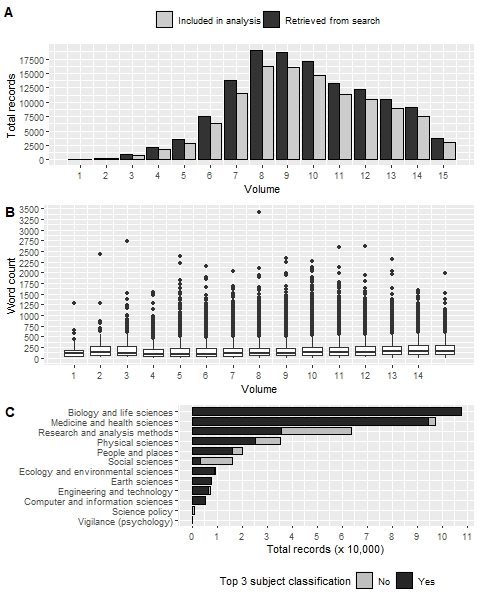
\includegraphics[width=0.8\linewidth]{figures/plossummary.jpg} 

}

\caption{\label{fig:plos-n} A: Search results by PLOS ONE volume; B: word count per statistical methods section included in analysis (n = 111,73); C: subject classifications assigned to full-text records included in analysis}\label{fig:unnamed-chunk-3}
\end{figure}

API searches returned 131,847 results (DOIs) based on chosen search
terms. After partial matching, 111,731 (85\%) statistical methods
sections were identified. In the final sample, 95,518 (85\%) DOIs
returned an exact match against common section headings: 64,133 for
`statistical analysis', 13,380 for `statistical analyses' and 13,627 for
`data analysis'. For our random sample of DOIs that did not meet the
partial matching criteria, initial search terms appeared in Introduction
(number), Results (number) only. xxx appeared in the Methods section
without a section heading and xxx had a non-standard section heading.
{[}TODO{]}.

Search results varied by journal volume (Figure \ref{fig:plos-n}A). The
total number of API search results peaked at volumes 8 (n = 19,045) and
9 (n = 19,045) in years 2013 and 2014. This trend aligned with the total
number of papers published in \emph{PLOS ONE} over the same period. The
percentage of records that included a statistical methods section by
volume based on our proposed matching criteria varied between 64\%
(volume 2) and 86\% (volume 9).

Statistical methods sections had a median length of 127 words and
inter-quartile range of 61 to 254 words (Figure \ref{fig:plos-n}B).
7,450 articles (7\%) had a statistical methods section of 500 words or
more. 19,461 articles (17\%) had sections with 50 words or less, equal
to the length of this paragraph.

All DOIs included Biology and life sciences (n = 107,584), Earth
sciences (n = 7,605) and/or Computer and information sciences (n =
5,190) in their top 3 subject classifications (Figure
\ref{fig:plos-n}C).

\begin{figure}

{\centering 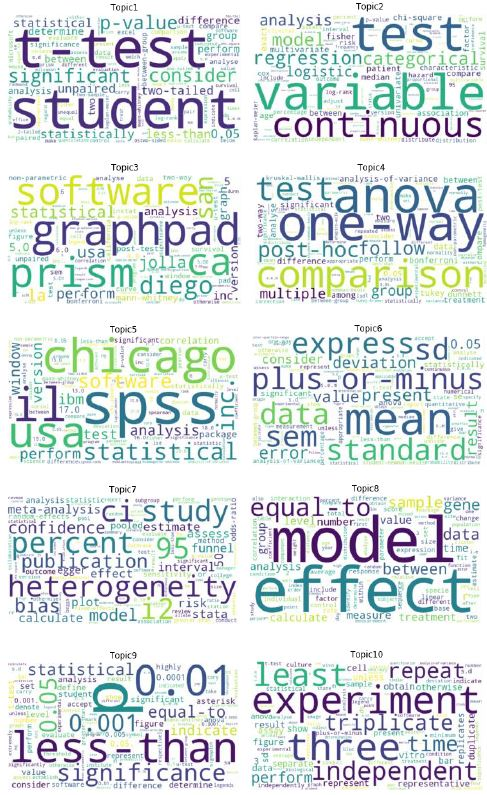
\includegraphics[width=0.8\linewidth]{figures/ploswordclouds.jpg} 

}

\caption{\label{fig:plos-clouds}Topic clouds for ten clusters for PLOS ONE}\label{fig:unnamed-chunk-5}
\end{figure}

The topic clouds based on ten clusters are in Figure
\ref{fig:plos-clouds}. Frequently occurring words reflected the use of
statistical software (topics 3 and 5), descriptive statistics (topic 6),
group based hypothesis testing (topics 1 and 4) and definitions of
statistical significance (topics 1 and 9). Statistical methods sections
related to regression (topic 2) and meta-analysis (topic 7) were also
identified.

Topics related to statistical software differentiated between Prism
GraphPad (topic 3: n = 9974; 8.6\%) and SPSS (topic 5: n = 9648; 8.3\%)
. Manual review of results showed that nine out of the ten top matching
DOIs for topic 3 stated the use of Prism GraphPad, but did not specify
which statistical methods were used. Top matching sections for topic 5
included information on SPSS version numbers and definitions of
statistical significance.

\begin{landscape}
\begin{table}

\caption{\label{tab:plos-example-boilerplate}Example boilerplate text from PLOS ONE dataset. Sentences marked with an asterisk $^{\dagger}$ correspond to the statistical methods section with the strongest match based on topic coherence score.}
\centering
\resizebox{1.15\textwidth}{!}{\begin{tabular}[t]{p{0.05\linewidth} p{0.80\linewidth} p{0.15\linewidth}}
\hline
Topic & Statistical methods text & Matching DOIs\\
\hline
1  & $^{\dagger}$Students t-test was used for statistical analysis & 29\\
 & $^{\dagger}$A p value of less-than 0.05 was considered statistically significant. & 1883\\
\cline{2-3}
 & Statistical analysis was performed using the students t-test & 380\\
  & p values of less-than 0.05 were considered significant. & 1526\\
\hline
3 & $^{\dagger}$GraphPad Prism (Graphpad Software, San Diego, CA) was used for all analyses. & 1941\\
\cline{2-3}
 & All statistical analysis was performed using Graphpad Prism software. & 1312\\
\hline
4 & $^{\dagger}$Significant differences were determined using analysis of variance (ANOVA) followed by Tukey post-hoc tests for multiple comparisons. & 2216\\
\cline{2-3}
 & Data are expressed as the mean ± SEM & 860\\
 & Statistical analysis was performed using one-way analysis of variance (ANOVA) test, followed by Dunnett’s multiple comparison post hoc test & 4516\\
 & P values less than 0.05 were considered significant & 2414\\
\hline
5 & $^{\dagger}$SPSS software version 17.0 (SPSS, Chicago, IL, USA) was used for statistical analysis. & 441\\
\cline{2-3}
 & The results are presented as the mean ± SEM. & 420\\
 & Data were analyzed by one-way ANOVA and LSD tests using the SPSS 13.0 software (SPSS Inc., Chicago, IL, USA). & 19\\
 & The difference was considered statistically significant at P$<$0.05. & 2555\\
\hline
6 & $^{\dagger}$All results are expressed as means ± standard deviation (± SD). & 102\\
\cline{2-3}
 & Data are expressed as mean ± Standard error of the mean (SEM) & 604\\
 & Statistical analysis of the data was performed by the Student’s t-test & 444\\
 & A value of P$<$0.05 was considered statistically significant. & 1786\\
\hline
9 & $^{\dagger}$Statistical significance was determined by Students t-tests. & 49\\
 & $^{\dagger}$$^{*} P<0.05$, $^{**} P = <0.01$, $^{***} P<0.001$. & 6\\
\cline{2-3}
 & Data are presented as the mean ± SD. & 378\\
 & Statistical analysis was performed using the Students unpaired t-test. & 752\\
 & Differences were considered statistically significant at $^{*}p<0.05$, $^{**}p<0.01$ and $^{***}p<0.001$. & 413\\

\hline
\end{tabular}}
\end{table}
\end{landscape}

Definitions of statistical significance featured strongly in topic 1 (n
= 3784; 3.2\%) and topic 9 (n = 6195; 5.3\%), combined with text
describing hypothesis testing for comparing differences between two
groups. Topic 1 reflected applications of Student's t-test assuming a
5\% level of statistical significance. Topic 9 referenced similar
methods combined with multiple thresholds for declaring statistical
significance by asterisk: ``\(^{*}p<0.05\), \(^{**}p<0.01\) and
\(^{***}p<0.001\)'', a practice that has been criticised
\citep{Wasserstein2019}.

Group-based hypothesis testing was a recurring theme across topics, with
text varying based on method(s) used. One-way analysis of
variance featured strongly in topic 4 (n = 10212; 8.8\%), combined
with common methods for performing post-hoc multiple comparisons, for example, Tukey's test and Dunnett's test.
Frequently occurring words in topic 6 (n = 4764; 4.1\%) reflected
mentions of descriptive statistics for summarising continuous variables,
for example: ``Data are expressed as means ± standard error of the mean
(SEM).'' Sections assigned to this topic appeared to be expanded
versions of topics 1 and 9. Examples of boilerplate text were in the
form of descriptive statistics followed by hypothesis testing, for
example, Student's t-test, Mann Whitney U or one-way analysis of
variance.

Examples of boilerplate text for selected topics are presented in Table
\ref{tab:plos-example-boilerplate}.

\subsection{ANZCTR}

We downloaded 28,008 studies. The numbers of excluded studies are shown
in Figure \ref{fig:anzctr-missing}. Of the 12,700 included studies,
9,523 (75\%) had a statistical methods section. The median length of
sections was 129 words with an inter-quartile range of 71 to 219 words.

We examined if four study characteristics were associated with a missing
statistics section. The odds ratios and 95\% credible intervals are in
Table \ref{tab:anzctr-missing-odds}. Observational studies were less
likely to have a missing methods section compared with interventional
studies. Missing sections became less likely over time. Studies with
more funders and a larger target sample size were less likely to have a
missing methods section.

\begin{table}[]
\centering
\caption{Regression results for factors associated with missing statistical methods sections in ANZCTR}
\label{tab:anzctr-missing-odds}
\begin{tabular}{lcc}
\hline
Variable & Odds ratio & 95$\%$ CI \\
\hline
Study type $=$ Observational & 0.78 & (0.69, 0.89) \\
Date (per year) & 0.90 & (0.88, 0.91) \\
Number of funders & 0.80 & (0.74, 0.86) \\
Target sample size (per doubling) & 0.90 & (0.88, 0.92)\\
\hline
\end{tabular}
\end{table}

\begin{figure}

{\centering 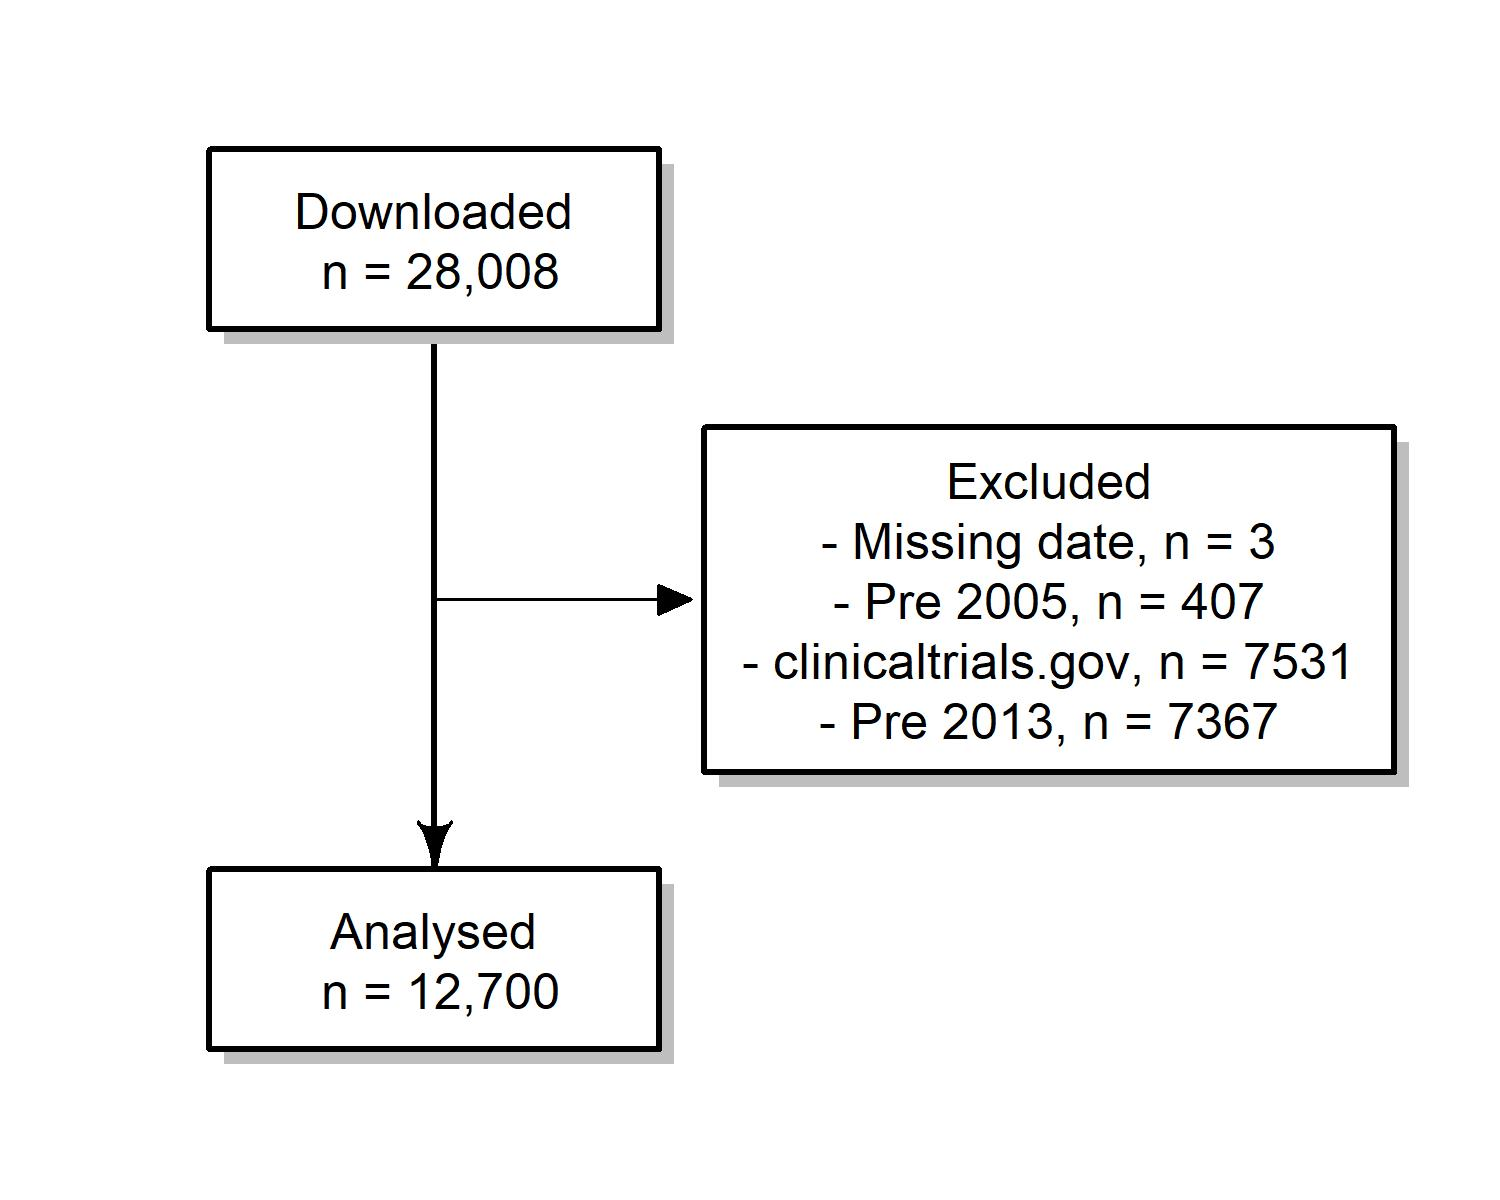
\includegraphics[width=0.7\linewidth]{figures/excluded_anzctr_missing} 

}

\caption{\label{fig:anzctr-missing}ANZCTR search results.}\label{fig:unnamed-chunk-8}
\end{figure}

\begin{figure}

{\centering 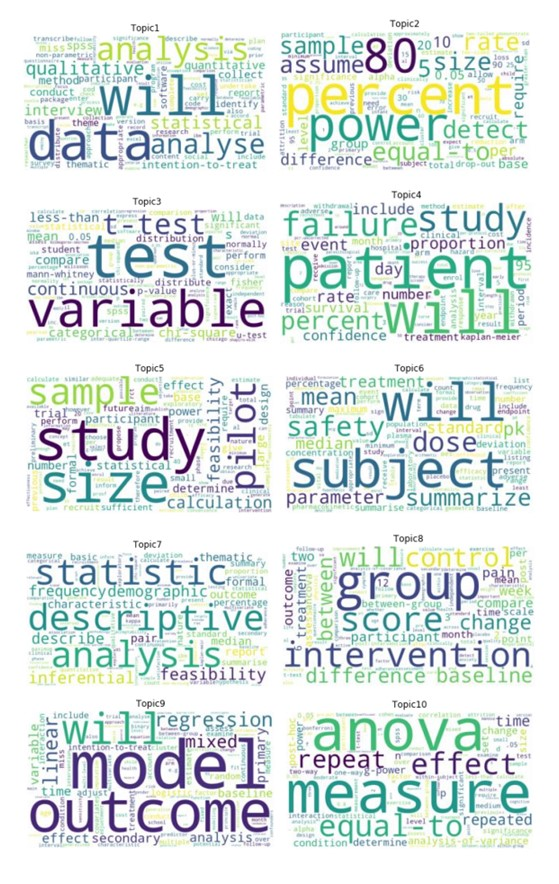
\includegraphics[width=0.7\linewidth]{figures/anzctrwordclouds} 

}

\caption{ANZCTR topic clouds.}\label{fig:unnamed-chunk-9}
\end{figure}

The clustering algorithm found groups that were purely sample size
calculations (topic 2, n = 1834; topic 4, n = 909), pilot studies (topic
5, n = 834), safety/tolerability studies (topic 6, n = 524),
intervention studies (topic 8, n = 1020) and repeated measures ANOVA
(topic 10 = 852). Examples of boilerplate text are provided in Table
\ref{tab:anzctr-example-boilerplate} and Supplementary File 3.

Some methods sections were only one word, including ``ANOVA'',
``t-test'', ``SPSS'' and even ``SSPS''. There were cases where the exact
same method section had been re-used in a different study. For example,
in topic 7 (n = 333), 232 sections stated `descriptive statistics' or
`descriptive statistics used' with no additional details provided. Other
instances with expanded descriptions of methods included topic 3 (n =
1277) outlining descriptive analyses only, and topic 6 (n = 524), for
hypothesis testing methods, statistical significance and software.

In other cases, text had been slightly modified to account for changes
in primary and secondary outcomes. Examples of these text changes were
found in topic 2 (n = 1834) and topic 4 (n = 909); identified instances
related to sample size calculations for patient recruitment to different
studies (see Supplementary File 3).

Targeted searches for the term `statistician' revealed
instances across all topics where no methods were specified. Instead,
all analyses were the responsibility of an appointed statistician, for
example, ``A statistician employed by hospital was used'' and ``Pilot
study at this point will use a statistician professionally to determine
sample size calculations as required''.

\begin{landscape}
\begin{table}[]
\centering
\caption{Example boilerplate text from ANZCTR dataset}
\label{tab:anzctr-example-boilerplate}
\begin{tabular}{p{0.1\linewidth} p{0.9\linewidth}}
\hline
\textbf{Topic} & \textbf{Statistical methods section} \\ \hline
3 & Comparisons between categorical variables will be made either using chi square or Fisher exact test. Continuous data will be compared using the Student’s t-test or Mann-Whitney U test. Two sided p values of less than 0.05 will be considered statistically significant.\\
 &  The Mann-Whitney U, Student t, 1-way ANOVA, and Kruskal-Wallis tests will be used to compare continuous variables where relevant. The Fisher exact and Pearson’s Chi-square test will be used to compare proportions as appropriate. \\ \hline
5 & Pilot study \\
 &  No formal sample size calculation was performed \\ \hline
7 & Descriptive statistics \\
 &  Descriptive statistics used \\ \hline
9 & Linear mixed models will be used to analyse the data. \\ \hline
10 & Repeated measures of ANOVA \\
 &  Pre-, during, post- and follow-up variables will be subjected to mixed methods and repeated measures analyses to determine significant changes over (group and) time. \\ \hline
\end{tabular}
\end{table}
\end{landscape}

\hypertarget{discussion}{%
\section{Discussion}\label{discussion}}

The first line in many statistical analysis sections in \emph{PLOS ONE}
was the software used and some entire sections in ANZCTR only stated the
software, implying that the software is the most important detail. As
Doug Altman said, ``Many people think that all you need to do statistics
is a computer and appropriate software'' \citep{Altman1994}. This is far
from the truth, and whilst it is important for researchers to mention
the software and version used for reproducibility purposes, it is a
minor detail compared with detailing what methods were used and why.

A frequent theme in the boilerplate statistical methods is the
definition of statistical significance, nearly always using a p-value at
the 5\% level. This widespread use of statistical significance is
troubling giving the bright-line thinking it engenders
\citep{McShane2019} and the common misinterpretations of p-values
\citep{Goodman2008}.

Despite the extensive array of statistical tests available, many authors
are reporting the same few methods.

One reason these inadequate sections get published is that most journals
do not use statistical reviewers, despite empirical evidence showing
they improve manuscript quality \citep{Hardwicke2020}.

A related paper has criticised vague statistical methods sections
because they deprive readers and reviewers for the opportunity to
confirm that the appropriate methods were used \citep{Weissgerber2018}.
These authors checked hundreds of papers using ANOVA and found that 95\%
did not contain the information needed to determine what type of ANOVA
was performed. This lack of information could well be because the
authors used a boilerplate statistical methods section that was missing
key details.

If authors shared their code then this would provide an alternative
route for checking what statistical methods were used. This is not a
perfect solution, as we still want authors to accurately report their
methods, but it does increase transparency. However, a recent paper
found that code sharing was very low in biomedical papers, with just 2\%
of a sample of over 6,000 papers sharing code \citep{Serghiou2021}.

Many researchers are using lazy practice by copying a standard
``boilerplate'' statistical methods section, likely cut-and-pasting from
other researchers or projects. This is a strong sign of the ritualistic
practice of statistics where researchers go through the motions rather
than using conscientious practice \citep{Stark2018}. This is concerning
because using the wrong statistical methods can reduce the value of
study, or worse, invalidate the entire study. These mistakes are
avoidable and are wasting of thousands of hours of researchers' time and
the time of patients and volunteers. Poor statistical practice is a key
driver of the ongoing reproducibility crisis in science
\citep{Ioannidis2014}.

\hypertarget{limitations}{%
\subsection{Limitations}\label{limitations}}

We did not check whether papers used the correct methods, and for some
simple studies a `boilerplate' statistical methods might be adequate.

We examined papers where there was a statistics section, and we missed
papers that used statistical analysis but did not include a statistical
analysis section. Reiterate outcomes of random sample checking here.

We only examined one large journal and one trial registry and hence our
results may not be generalisable to all journals or registries,
especially those that consistently use a statistical reviewer.

We searched the full text of \emph{PLOS ONE} papers but not the
supporting information which may contain statistical methods sections
for some papers. The search terms we used to find statistical methods
appeared in the supporting information titles for xxx papers (x\%). We
did not include the supporting information because it is less structured
than the paper and could be in PDF or Word format.

\bibliographystyle{agsm}
\bibliography{references.bib}

\end{document}
